% !TEX TS-program = pdflatex
% !TEX encoding = UTF-8 Unicode

% This is a simple template for a LaTeX document using the "article" class.
% See "book", "report", "letter" for other types of document.

\documentclass[11pt]{article} % use larger type; default would be 10pt

\usepackage[utf8]{inputenc} % set input encoding (not needed with XeLaTeX)

%%% Examples of Article customizations
% These packages are optional, depending whether you want the features they provide.
% See the LaTeX Companion or other references for full information.

%%% PAGE DIMENSIONS
\usepackage{geometry} % to change the page dimensions
\geometry{a4paper} % or letterpaper (US) or a5paper or....
\geometry{margin=0.75in} % for example, change the margins to 2 inches all round
% \geometry{landscape} % set up the page for landscape
%   read geometry.pdf for detailed page layout information

\usepackage{graphicx} % support the \includegraphics command and options

% \usepackage[parfill]{parskip} % Activate to begin paragraphs with an empty line rather than an indent

%%% PACKAGES
\usepackage{booktabs} % for much better looking tables
\usepackage{array} % for better arrays (eg matrices) in maths
\usepackage{paralist} % very flexible & customisable lists (eg. enumerate/itemize, etc.)
\usepackage{verbatim} % adds environment for commenting out blocks of text & for better verbatim
\usepackage{subfig} % make it possible to include more than one captioned figure/table in a single float
\usepackage{hyperref}
\usepackage{float}
\hypersetup{
    colorlinks=true,
    linkcolor=blue,
    filecolor=magenta,      
    urlcolor=cyan,
    pdftitle={Overleaf Example},
    pdfpagemode=FullScreen,
    }
\usepackage{listings}
\usepackage{minted}
\usepackage{hyperref}


% These packages are all incorporated in the memoir class to one degree or another...

%%% HEADERS & FOOTERS
\usepackage{fancyhdr} % This should be set AFTER setting up the page geometry
\pagestyle{fancy} % options: empty , plain , fancy
\renewcommand{\headrulewidth}{0pt} % customise the layout...
\lhead{}\chead{}\rhead{}
\lfoot{}\cfoot{\thepage}\rfoot{}

%%% SECTION TITLE APPEARANCE
\usepackage{sectsty}
\allsectionsfont{\sffamily\mdseries\upshape} % (See the fntguide.pdf for font help)
% (This matches ConTeXt defaults)

%%% ToC (table of contents) APPEARANCE
\usepackage[nottoc,notlof,notlot]{tocbibind} % Put the bibliography in the ToC
\usepackage[titles,subfigure]{tocloft} % Alter the style of the Table of Contents
\renewcommand{\cftsecfont}{\rmfamily\mdseries\upshape}
\renewcommand{\cftsecpagefont}{\rmfamily\mdseries\upshape} % No bold!
\usepackage[numbers]{natbib}
%\renewcommand{\thepage}{S\arabic{page}}
%\renewcommand{\thesection}{S\arabic{section}}
%\setcounter{table}{0}
%\renewcommand{\thetable}{Table \arabic{table}}
%\setcounter{figure}{0}
%\renewcommand{\thefigure}{Figure \arabic{figure}}
%%% END Article customizations

%%% The "real" document content comes below...

\title{Solution of 2nd Place Logloss and 3rd Place Efficiency of Feedback Prize - Predicting Effective Arguments (Team SKT)}
\author{Shujun He, Tomohiro Takesako\footnote{Refered to as Tom later on}, and Kossi Neroma\footnote{Authors are listed in alphabetical order}}
%\date{} % Activate to display a given date or no date (if empty),
         % otherwise the current date is printed 

\begin{document}
\maketitle

\section{Background of our team}

We participated in the recent competition "Feedback Prize - Predicting Effective Arguments", which was hosted during the third quarter of 2022. Our team name is SKT. Our public leaderboard score is 0.55306 (2nd) and our private score is 0.55453 (2nd). We also rank 3rd on the efficiency leaderboard with an efficiency score of 1.055925. 

Our team consistes of Shujun, who is a PhD student in chemical engineering at Texas A\&M University in College Station, TX, US, Tom, who is a data scientist at Sprout.ai, and Kossi Neroma, who is a junior data scientist at Publicis Sapient. 

\section{Solution overview}
Each of our team members has their own training pipeline for transformer models. On a high level, our transformer models look at the entirety of each essay and output predictions of effectiveness for each discourse either via pooling of discourse tokens or a classification token added to the front of the each discourse. Importantly, directly inputting essays results in a situation where the model is not sure about where it needs to make predictions, so to circumvent this, we use either a prompt (i.e. concat f'(\{discourse\_type\} start)' and f'(\{discourse\_type\} end)' to the beginning and end of each discourse to signal where predictions need to be made) or simply concat special tokens added to the tokenizer instead (i.e. f' [discourse\_type]' and f'[discourse\_type\textbackslash ]') (\autoref{fig: example}). Following training of transformer models, we also use stacking models (e.g. xgboost) to further improve predictions. Further, we utilize unlabled data from the previous Feedback competition in a semi-supervised (i.e. pseudo-labeling) setting. 

\begin{figure}[H]
\center
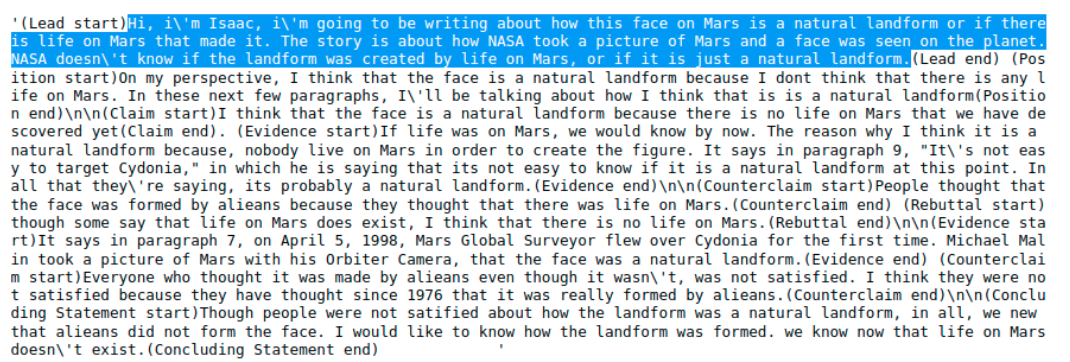
\includegraphics[width=0.9\textwidth]{graphics/example_segments.png}
\caption{Example of a preprocessed essay. The first discouse is segmented by prompts and highlighted. }
\label{fig: example}
\end{figure}


\section{Transformer modeling}
\subsection{Encoders}
Deberta  \cite{DBLP:journals/corr/abs-2006-03654, DBLP:journals/corr/abs-2111-09543} worked the best since it supports unlimited input length and uses disentangled attention with relative positional embedding; in fact, our ensemble consists entirely of deberta variants. For Shujun, it was also helpful to add a GRU/LSTM after pooling on the pooled discourse representations. Tom used Shujun's SlidingWindowTransformerModel from the last Feedback competiion (\url{https://www.kaggle.com/competitions/feedback-prize-2021/discussion/313235}), which stablized training for him.

\subsection{Pretraining}
Kossi used pretrained weights from his solution in the last competiion (\url{https://www.kaggle.com/competitions/feedback-prize-2021/discussion/313478}) and Tom and I found pretrained tascj0 models to be good starting points. We used some of the weights that tascj0 released after the last Feedback competition and Tom also pretrained some new ones on his own. Please checkout out tascj0's solution post if you'd like to learn more (\url{https://www.kaggle.com/competitions/feedback-prize-2021/discussion/313424}).
In addition, Tom used MLM for some of his models. Further, some of our models simply used huggingface weights.

\subsection{Max sequence length}
Shujun used a max sequence length of 1280 in both training and inference, since he found that 99.9\% of discourses fall within that range, whereas other teammates used up to around 1800 during inference and as low as 648 in training.

\section{Pseudo labeling}
Pseudo labeling is an integral part of all our solution. We use essays from the training set of last Feedback competition that are also not present in the training set of this competition. Our procedure is as follows:

\begin{enumerate}

\item Train model with gt labels
\item Make predictions for old data (around 11000 essays) with each fold model
\item Retrain model with crossentropy on pseudo label probabilities (not discretized) generated by previous model trained on the same fold data: 3 epochs on pl labels only first and then 3 more epochs on gt labels only
\item Repeat from step 2
\end{enumerate}

For Shujun's pipeline, I saw improvement until 5 rounds of the above procedure. For Tom, it was only helpful for one round and Kossi did not have enough time to try multi-round pl.

\section{Stacking}
Stacking provides significantly improvement in both cv/lb (around 0.004). Our stacking framework is primarily inspired by my team's solution (\url{https://www.kaggle.com/competitions/feedback-prize-2021/discussion/313235}) in the previous feedback competition. In addition to predicted probabilities outputted by the transformer models, we also utilized the token probabilities for each discourse, which we call prob\_sequences. Compared to the previous Feedback competition, stacking is much faster since we don't have to deal with a huge amount of candidate sequences. Our features are as follows:

\begin{minted}[mathescape, linenos,fontsize=\footnotesize]{python}

def get_xgb_features(train_df,prob_sequences):
    features2calculate=[f"instability_{i}" for i in range(4)]+\
    [f"begin_{i}" for i in range(3)]+\
    [f"end_{i}" for i in range(3)]#+\
    #["entropy"]

    calculated_features=[]
    for i,prob_seq in tqdm(enumerate(prob_sequences)):

        tmp=[]
        #quants = np.linspace(0,1,n_quan)
        prob_seq=np.array(prob_seq)
        instability = []
        #all_quants=[]
        tmp.append(np.diff(prob_seq[:,:],0).mean(0))
        tmp.append([(np.diff(prob_seq[:,[1,2]].sum(1))**2).mean()])

        tmp.append(prob_seq[:5,:].mean(0))
        tmp.append(prob_seq[-5:,:].mean(0))

        calculated_features.append(np.concatenate(tmp))


    train_df[features2calculate]=calculated_features
    train_df['len']=[len(s) for s in prob_sequences]

    calculated_features=np.array(calculated_features)
    calculated_features.shape

    p_features=[]
    n_features=[]
    neighbor_features=['Ineffective','Adequate','Effective','discourse_type']
    neighbor_features_values=train_df[neighbor_features].values
    for i in tqdm(range(len(train_df))):
        if i>1 and train_df['essay_id'].iloc[i]==train_df['essay_id'].iloc[i-1]:
            p_features.append(neighbor_features_values[i-1])
        else:
            p_features.append(neighbor_features_values[i])

        if i<(len(train_df)-1) and train_df['essay_id'].iloc[i]==train_df['essay_id'].iloc[i+1]:
            n_features.append(neighbor_features_values[i+1])
        else:
            n_features.append(neighbor_features_values[i])

    train_df[[f+"_previous" for f in neighbor_features]]=p_features
    train_df[[f+"_next" for f in neighbor_features]]=n_features

    train_df['mean_Ineffective']=train_df.groupby("essay_id")["Ineffective"].transform("mean")
    train_df['mean_Adequate']=train_df.groupby("essay_id")["Adequate"].transform("mean")
    train_df['mean_Effective']=train_df.groupby("essay_id")["Effective"].transform("mean")

    train_df['std_Ineffective']=train_df.groupby("essay_id")["Ineffective"].transform("std")
    train_df['std_Adequate']=train_df.groupby("essay_id")["Adequate"].transform("std")
    train_df['std_Effective']=train_df.groupby("essay_id")["Effective"].transform("std")

    train_df['discourse_count']=train_df.groupby("essay_id")['discourse_type'].transform("count")

    cnts=train_df.groupby('essay_id')['discourse_type'].apply(lambda x: x.value_counts())

    #new_df=[]
    discourse_types=['Claim','Evidence','Concluding Statement','Lead','Position','Counterclaim','Rebuttal']
    value_count_hash={}
    for t in discourse_types:
        value_count_hash[t]={}
    for key in cnts.keys():
        value_count_hash[key[1]][key[0]]=cnts[key]

    discourse_cnts=[]    
    for essay_id in train_df['essay_id'].unique():
        row=[essay_id]
        for d in discourse_types:
            try:
                row.append(value_count_hash[d][essay_id])
            except:
                row.append(0)
        discourse_cnts.append(row)

    discourse_cnts=pd.DataFrame(discourse_cnts,columns=['essay_id']+[f'{d}_count' for d in discourse_types])    
    #discourse_cnts

    train_df=train_df.merge(discourse_cnts,how='left',on='essay_id')
    train_df

    #train_df

    return train_df

\end{minted}
Since stacking is fast, it works best when we use each fold predictions with xgb separately and then avg. For instance, because Shujun has 6 folds of neural network models and 6 folds of xgb models, this way he has 6x6=36 preds to avg for each single model.

\section{Best single models}
All our best single models were deberta-large/deberta-v3-large variants. For Tom and Kkiller, their best single models came from 1st round PL, whereas for Shujun it came from 4th round PL (\autoref{tab: single models}).

\begin{table}[H]
\center
\begin{tabular}{|c|c|c|c|}
\hline
           & Shujun         & Tom   & Kkiller \\ \hline
Public LB  & \textbf{0.560} & 0.566 & 0.562   \\ \hline
Private LB & \textbf{0.558} & 0.571 & 0.562   \\ \hline
Local CV   & 0.571          & N/A   & 0.572   \\ \hline
\end{tabular}
\caption{Best single models of team SKT. }
\label{tab: single models}
\end{table}

\section{Ensemble}

Our final submission is a weighted average of best ensembles from each individual member (\autoref{tab: ensemble}). For Shujun, his best ensemble consists of 6 folds of (5th round pseudo-labeling models):
\begin{enumerate}
\item deberta-v3-large (tascj0 span detector pretrained)
\item deberta-v2-xlarge (tascj0 span detector pretrained)
\item deberta-v1-xlarge (tascj0 span detector pretrained)
\item deberta-v3-large (huggingface pretrained)
\item deberta-v2-xlarge (huggingface pretrained)
\end{enumerate}


For Tom, his best ensemble consists of 5 folds of:
\begin{enumerate}
\item deberta-large (tascj0 span detector pretrained, 2nd round pseudo-labeling model, stacking not applied)
\item deberta-v3-large (tascj0 span detector pretrained, 2nd round pseudo-labeling model, stacking not applied)
\item deberta-large (tascj0 span detector pretrained, 1st round pseudo-labeling model)
\item deberta-v3-large (tascj0 span detector pretrained, 1st round pseudo-labeling model)
\end{enumerate}

For Kkiller, hist best ensemble consists of 5 folds of:
\begin{enumerate}
\item deberta-large (kkiller pretrained + psl + shujun stacking)
\item deberta-v3-large (kkiller pretrained + psl + shujun stacking)
\item deberta-xlarge (kkiller pretrained + psl  + shujun stacking)
\item deberta-v2-xlarge (kkiller pretrained + + psl + shujun stacking)
\end{enumerate}

\begin{table}[H]
\center
\begin{tabular}{|c|c|c|c|c|}
\hline
                                                                   & Shujun           & Tom     & Kkiller & Ensemble \\ \hline
Public LB                                                          & \textbf{0.55727} & 0.56190 & 0.55931 & 0.55306  \\ \hline
Private LB                                                         & \textbf{0.55538} & 0.56648 & 0.56245 & 0.55453  \\ \hline
\begin{tabular}[c]{@{}c@{}}Weight in\\ final ensemble\end{tabular} & 0.45             & 0.25    & 0.3     &          \\ \hline
\end{tabular}
\caption{Best ensembles of team SKT. }
\label{tab: ensemble}
\end{table}


\section{Efficiency submission}
Our efficiency model is the same as Kossi's deberta-v3-large mentioned above except that it was trained on all the data (psl + ground truth) for 3 epochs. For faster inference, Kossi also includes a [trunc...] token which allows to have a max length under 1024 whith no decrease in performance. Therefore, all discourses under the max length are taken into account and discourses appearing after max length are truncated. For all Kossi's models, discourse-pooling  (when applied, otherwise a custom classification token) occurs before softmax.

\section{Some more tips/tricks}
For Tom AWP was useful, and he reported around 0.003 cv improvement with AWP (eps=1e-3 and lr=1e-2 for large models, 1e-4 for xlarge models).

It was also important to split the data with StratifiedGroupKFold instead of GroupKFold. For me I started out with GroupKFold but found better correlation between cv/lb after switching to StratifiedGroupKFold.

For ensembling models with the same cv split, we used GP\_minimize (from sklearn) to find optimal weights and otherwise weights were determined arbitrarily.

Gradient accumulation was useful since we had to deal with very long sequences.

\bibliographystyle{plain} % We choose the "plain" reference style
\bibliography{references} % Entries are in the refs.bib file


\end{document}
